\section{问题二}
\subsection{问题重述}
调研为什么常用的同轴线特性阻抗为$50$欧姆和$75$欧姆,它们各自应用在什么领域?
\subsection{回答问题}
射频同轴电缆在RF中通常选用$50$欧姆作为标准有几方面的原因:一是功率容量,抗击穿电压与衰减之间的综合考虑;
二是机械美观上的考虑。
设同轴线的绝缘层是空气介质,其相对介电常数为1,同轴线的阻抗值为:
\begin{equation}\label{10}
    Z_0=\sqrt{\frac{R+\jmath\omega L}{G+\jmath\omega C}}
\end{equation}
当$R\ll \omega L$,$G\ll \omega C$ 时,可对上述公式做以简化:
其中: $D$为外导体直径,$d$ 为内导体直径。
\subsubsection{最大功率容量}
若想在信号传输过程中有望得到最大功率容量,即 $P_{\max}$:
\begin{equation}\label{12}
    P_{\max}=\dfrac{V_{\max}^2}{Z_0}\propto \dfrac{Ed\ln\frac{D}{d}}{Z_0}
\end{equation}
将$Z_0$代入上式,有:
\begin{equation}\label{13}
    P_{\max}\propto \dfrac{E^2d^2\ln\frac{D}{d}}{60}
\end{equation}
对式\ref{13}求导并令求导结果为零,可求得极值,得出$\dfrac{D}{d}=1.6$,
此时,同轴线的阻抗为$30\Omega$ 。
\subsubsection{最小衰减}
在信号传输过程中希望有最小的衰减,即:
\begin{equation}\label{14}
    \alpha_{\min}=\alpha_R+\alpha_G
\end{equation}
其中$\alpha_R$为导体电阻损耗引起的电缆衰减分量,称为导体衰减;
$\alpha_G$ 为绝缘介质损耗引起的电缆衰减分量,称为介质衰减。
由于假设绝缘层介质为空气,因此只考虑导体衰减分量$\alpha_R$ 。
\begin{equation}\label{15}
    \alpha_R=\dfrac{R}{2Z_0}
\end{equation}
其中$R$为电缆的总趋肤效应串联电阻之和,同轴电缆内导体趋肤效应电阻与内导体直径$d$
成反比,屏蔽层趋肤效应电阻与外导体直径$D$成反比,有:
\begin{equation}\label{16}
    R=\dfrac{\dfrac{1}{D}+\dfrac{1}{d}}{2\pi\delta\sigma}
\end{equation}
代入式\ref{15}可得:
\begin{equation}
    \alpha_R\propto \dfrac{\dfrac{1}{D}+\dfrac{1}{d}}{\ln\dfrac{D}{d}}
\end{equation}
对上式求导,令求导结果为$0$,可求得极值。当$\dfrac{D}{d}=3.6$时,$\alpha_R$最小,
此时同轴线的阻抗为$77\Omega$。

\textbf{综合功率传输量与衰减两方面的考虑,取折中即50欧姆。通过实践发现,50欧姆的系统阻
    抗,对于半波长偶极子天线和四分之一波长单极子天线的端口阻抗也是匹配的,引起的反
    射损耗是最小的。}

另外,以上计算是假设绝缘层为空气时计算得出的结果,实际应用中,绝缘层通常采用聚
乙烯材料,其相对介电常数为$2.3$。此时特性阻抗为:
\begin{equation}\label{18}
    Z`_0=\dfrac{Z_0}{\sqrt{\varepsilon_r}}=50.77
\end{equation}

近似就是常见的同轴线特性阻抗\textbf{50欧姆}。并不是每个高频系统或组件都针对50欧姆设计的。
75欧姆阻抗仍然很常见;同轴电缆的特性阻抗与其外径$D$与内径$d$之比的自然对数成正比。
这意味着内部导体和外部导体之间的更大间隔对应于更高的阻抗。两个导体之间的较大间距也
导致较低的电容。因此,75欧姆的同轴电缆的电容比50欧姆同轴电缆的电容更低,这使75欧
姆电缆更适合于高频数字信号,因为这种信号需要低电容,以避免与逻辑低和逻辑高之间的
快速过渡相关的高频内容过度衰减。

下通过使用Matlab编程给出功率容量和衰减随特性阻抗的变化曲线,如图\ref{pic2-1}所示。
\begin{figure}[htbp]
    \centering
    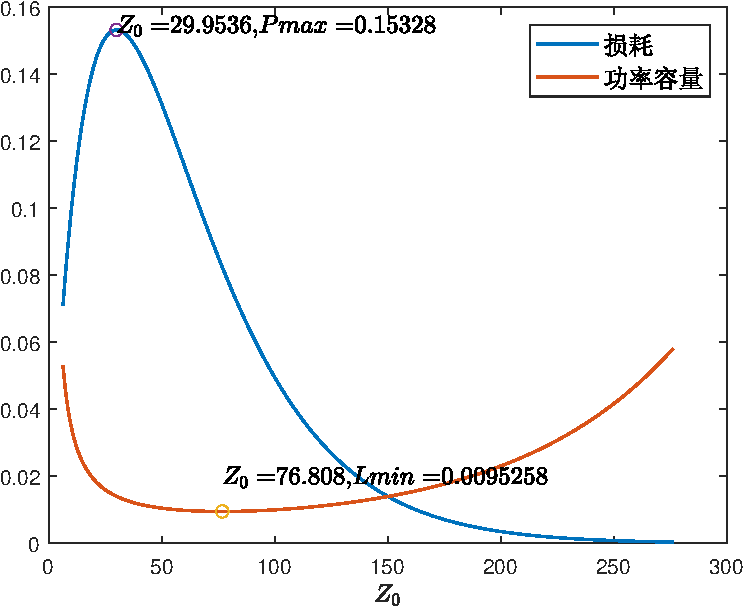
\includegraphics[width=0.7\linewidth]{figure/microwave-crop.pdf}
    \caption{功率容量和损耗随特性阻抗变化曲线}
    \label{pic2-1}
\end{figure}
\subsection{机械美观}
为了减小电缆的衰减而提高电缆的阻抗$Z_0$ ,中心内导体的直径$d$ 相对于整个电缆直径来说要相当细
才可以。为降低电缆的特征阻抗,内导体和屏蔽层之间的绝缘介质的厚度要做的很薄。这样几乎
所有的电缆为了机械上的美观其特征阻抗都会接近50欧姆,这也使得50欧姆特征阻抗成为标准的
一个自然趋势。
\subsection{应用领域}
我们常见的系统中,比如电视TV和广播FM接收系统中,其系统阻抗基本上都是75欧姆,因为75欧姆
射频传输系统中,信号传输的损耗是最小的,TV和广播FM接收系统中,信号的传输损耗是重要的考
虑因素。而对于带有发射的电台而言,50欧姆是很常见的,因为最大功率传输是我们考虑的主要因
素,同时损耗也比较重要。这就是为什么我们的对讲机系统中,经常看到的都是50欧姆的参数指标。

在有些设计中上面两个阻抗极点也是极其重要的。比如在同轴滤波器设计中,我们希望同轴谐振器
的损耗最低,那就需要用到$ Z=77\Omega$这个阻抗。这时候的同轴线内外半径比为$D/d=3.6$时,谐振腔的损耗最低。
当然如果功率容量时设计瓶颈的话,会用到Z=30Ohm这个阻抗。这个时候同轴线的外径内径比为:D/d=1.6。

\textbf{结语:工程设计本身就是一个平衡的过程,我们平衡性能,工艺,成本。我们根据系统的需要去做
    有效的平衡。这本身就贯穿射频工程设计的各个阶段。}
